\documentclass[a4paper,10pt]{article}
\usepackage[utf8]{inputenc}
\usepackage{graphicx}
\usepackage{xcolor}
\usepackage{listings}
\graphicspath{ {./graphs/} }
\graphicspath{ {./code/} }

\definecolor{mGreen}{rgb}{0,0.6,0}
\definecolor{mGray}{rgb}{0.5,0.5,0.5}
\definecolor{mPurple}{rgb}{0.58,0,0.82}
\definecolor{backgroundColour}{rgb}{0.95,0.95,0.92}

\lstset{extendedchars=\true}
\lstset{inputencoding=ansinew}

\lstdefinestyle{CStyle}{
    backgroundcolor=\color{backgroundColour},   
    commentstyle=\color{mGreen},
    keywordstyle=\color{magenta},
    numberstyle=\tiny\color{mGray},
    stringstyle=\color{mPurple},
    basicstyle=\footnotesize,
    breakatwhitespace=false,         
    breaklines=true,                 
    captionpos=b,                    
    keepspaces=true,                 
    numbers=left,                    
    numbersep=5pt,                  
    showspaces=false,                
    showstringspaces=false,
    showtabs=false,                  
    tabsize=2,
    language=C
}


\title{\textbf{Operativsystem ID1206} \\ 
\textbf{Gröna trådar}}

\author{Axel Karlsson}

\begin{document}

\maketitle
\textbf
    {\\\\1. Inledning\\\\}
I denna rapport har jag redovisat mitt arbete med seminarieuppgift 3, Green, i kursen ID1206 Operativsystem. Uppgiften var att implementera ett trådbibliotek likt c-biblioteket ``pthreads''.  I del 2 har jag redovisat min implementation och i del 3 har jag jämfört mitt bibliotek med pthreads.

\maketitle
\textbf
{\\1.2 Vad är ett trådbibliotek?\\}
Ett trådbibliotek är, som man hör på namnet, ett bibliotek som ger oss möjlighet att skapa och köra trådar i ett program. Att programmera med flera trådar är inte ett lätt jobb och därför finns det även funktioner som låter oss (till viss del) styra hur dessa trådar exekverar, och på så sätt kan vi förhoppningsvis skriva ett buggfritt program. Mitt biblioteks api är baserat på pthreadbiblioteket och jag har implementerat följande funktioner:
\begin{itemize}
  \item pthread\_create() \& \_yield() \& \_join()
  \item pthread\_mutex\_lock() \& \_unlock() \& \_init()
  \item pthread\_cond\_init() \& \_wait() \& \_signal()
\end{itemize}

\maketitle
\textbf
    {\\2. Implementation\\\\}
    En stor del av koden till denna uppgift var given i instruktionerna och jag har försökt att inte ha med de delarna i rapporten. Detaljerna i min implementation blir som en konsekvens av det svåra att förstå om man själv inte har gjort uppgiften.
    
\maketitle
\textbf
{\\2.1 Hantera kontexter\\}
Den första delen av api:n jag implementerade var green\_create(), green\_yield() och green\_join(). De fyller samma funktion som pthreadfunktionerna med liknande namn; create() initierar en ny tråd, yield() flyttar den tråden som körs och lägger den längst bak i exekveringskön och join() suspenderar den tråden som körs tills en given tråd har terminerat.\\\\
Trådar som  är redo att exekveras läggs i en kö ``ready queue'' som jag valde att implementera som en länkad lista, med next pekaren i green\_t strukturen. \\\\
Den största utmaningen med denna del av uppgiften var för mig att implementera den interna funktionen green\_thread() på ett korrekt sätt. Funktionens syfte är kort sagt att ta trådar från ready-kön, exekvera dem och sedan terminera dem. När jag först skrev denna funktion förstod jag inte hur den hängde ihop med resten av programmet och jag har därför haft många buggar som härstammar från denna funktion.

\begin{lstlisting}[style=CStyle]
  void green\_thread() {
    ...
    // Denna if sats var lange ett fragetecken for mig
    if(this->join != NULL) {
      queue\_add(this->join, readyqueue);
    }
    ...
    
    green_t* next = queue\_remove(readyqueue);
    runnign = next;
    setcontext(next->context);

\end{lstlisting}

% skriv lite kodexempel här. Det mest intressanta är green_thread() & kön. Resten är samma för alla.

\maketitle
\textbf
{\\2.2 Conditional variables\\}
I denna del av uppgiften implementerade jag villkorliga variabler. En tråd exekverar tills den hamnar vid en villkorlig variabel, och blir då suspenderad tills variablen signal funktion anropas och tråden väcks igen. Api:n för dessa är cond\_init(), cond\_wait \& cond\_signal(). I min implementation finns green\_cond\_t structen, som skapas med init(). Den innehåller en länkad lista med trådar som väntar på variablen. Vi kan sedan lägga till eller ta bort trådar i denna lista med wait respektive signal, och på så sätt suspendera eller väcka dem. Jag hade ingen stor svårighet med denna del av uppgiften.

\begin{lstlisting}[style=CStyle]
  typedef struct green_cond_t {
    green_t* suspended_list; // Lankad lista som haller koade tradar
    } green_cond_t;

\end{lstlisting}
  
% Beskriv suspend grejen. Här är allt skrivt själv så kan beskriva rätt mycket

\maketitle
\textbf
    {\\2.3 Timer interrupt\\}
I denna del implementerade jag timerinterrupts av trådarna. Varje 100 millisekunder anropas en funktion som liknar yield, i att den sätter tråden som körs längst baj u exekveringskön och startar nästa. Detta möjliggör samtida (concurrent) exekvering av flera trådar utan att de explicit behöver släppa fram varandra (till exempel genom att anropa yield). Att byta tråd på fel ställe i programmet kan orsaka buggar och därför har även delar av koden ``skyddats'' från timerinterrupts.\\\\
I denna del var nästan all kod given i instruktionerna, det enda problemet var att tänka ut vilken kod som skulle skyddas från timerinterrupts. Min tankeprocess var att skydda all kod som ändrar i någon lista eller en global pekare, och det blev i princip all kod.

%Beskriv vad som är skyddat kanske, men det mesta är givet i instruktionen
 
\maketitle
\textbf
{\\2.4 Mutex\\}
Det sista jag implementerade var en mutex funktionalitet. Mutex låter oss placera ``lås'' i koden som trådar kan låsa eller låsa upp, och kort sagt kan vi se till att vissa delar av kod endast exekveras av en tråd i taget. \\\\
Även i denna del var majoriteten av koden given i uppgiften. Jag implementerade suspended-kön med en länkad lista lik den i green\_cond\_t strukturen. Api:n implementerad här är green\_mutex\_init(), green\_mutex\_lock() \& green\_mutex\_unlock().

% Det mesta är givet, beskriv tanken bakom typ. Nämn lista api någon annan stans.

\maketitle
\textbf
    {\\  2.5 Förbättring av green\_cond\_wait()\\}
    Denna del var svår. Målet var att implementera en funktion som kan vänta på ett lås tills en signal kommer, och sedan ta det låset. Detta är i princip en kombination av tidigare skrivna funktioner, men det är viktigt att ha dem i samma funktion (som en atomär operation) för att de inte ska bli avbrutna av timerinterrupt. Jag hade till en början svårt att förstå vad syftet med denna funktion var, men när jag förstod att det egentligen är en kombination av funktionaliteten i green\_cond\_wait() och mutex var det inte så svårt.
    
    \begin{lstlisting}[style=CStyle]
      green_cond_wait(cond, mutex) {
        // Forsta delen av den tidigare cond_wait()
        if(mutex != NULL) {
          // I princip mutex_unlock()
          ...
        }
        // Resten av den tidigare cond_wait()
        ...
        if(mutex != NULL) {
          // I princip mutex_lock()
        }
        return;
      }
    \end{lstlisting}
  
    
% Samma ganska given. beskriv lite svårigheter kanske
    \maketitle
    \textbf
{\\\\3. Benchmarks\\}
Jag har jämfört exekveringstid av de benchmark-funktioner jag har skapat med både pthreadbiblioteket och mitt bibliotek, se kodexempeln nedan. Varje benchmark har körts med två trådar samtidigt och antalet iterationer (variablen i) har testats mellan 100 och 3000 i intervall av 100.
\maketitle
\textbf
    {\\3.1 yield() benchmark\\}
    I detta benchmark anropartrådarna yield varje iteration.
    \begin{lstlisting}[style=CStyle]
      void* bmark_yield(int i) {
        ...
        while(i > 0) {
          fib(10); // Rakna 10:e fibbonaccitalet
          i--;
          yield(); // Detta ar pthread eller mitt bibliotek
        }
      }
    \end{lstlisting}
    
    \begin{figure}[htp]
      \centering
      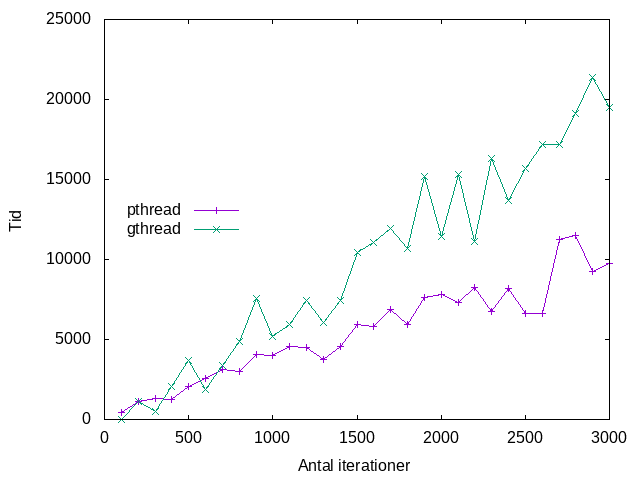
\includegraphics[width=8cm]{benchmarks/yieldtest.png}
      \caption{bmark\_yield(): Exekveringstid(ticks) / Iterationer}
      \label{fig:Graph}
    \end{figure}
    % Den viktigaste delen typ
    
    \maketitle
    \textbf
        {\\3.2 Timerbenchmark\\}
        I detta benchmark låter vi timerinterrupts byta mellan trådar.
            \begin{lstlisting}[style=CStyle]
      void* bmark_timer(int i) {
        ...
        while(i > 0) {
          fib(10); // Rakna 10:e fibbonaccitalet
          i--;
        }
      } \end{lstlisting}
         \begin{figure}[htp]
           \centering
           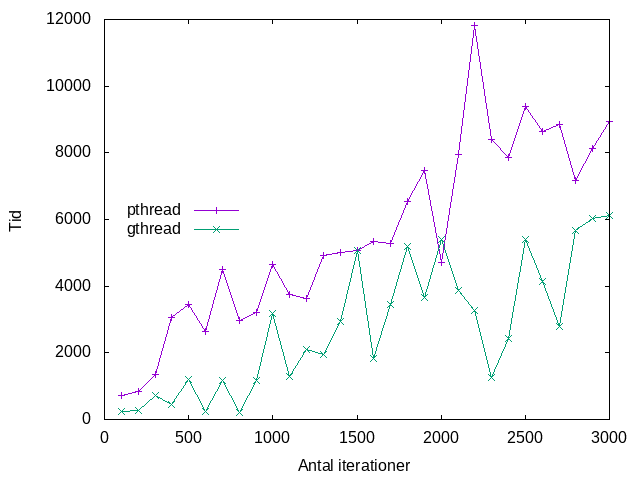
\includegraphics[width=8cm]{benchmarks/timertest.png}
           \caption{bmark\_timer(): Exekveringstid(ticks) / Iterationer}
           \label{fig:Graph}
         \end{figure}
         
         \maketitle
         \textbf
             {\\3.3 Mutexbenchmark\\}
             I detta benchmarks itereras en global variabel, som är skyddad av ett lås och en flagga. Detta test är samma som det givet i uppgiftinstruktionerna i del 6. Jag har försökt skriva testet i pseudokod, för en mer detaljerad beskrivning hänvisar jag till uppgiftinstruktionerna sida 11.
             \begin{lstlisting}[style=CStyle]
               void* bmark_mutex(int i) {         
                 while(i > 0) {
                   mutex_lock(&lock1);
                   while(flag != id) {
                     // En trad ar fast har
                     cond_wait(&cond1, &lock1);
                   }
                   flag = *den andra traden*
                   counter++;
                   fib(10); // Rakna 10:e fibonaccitalet
                   // Den andra traden slapps forbi cond_wait()
                   cond_signal(&cond1);
                   mutex_unlock(&lock1);
                   lim--;
                 }
               }
             \end{lstlisting}
             
             
        \begin{figure}[htp]
          \centering
          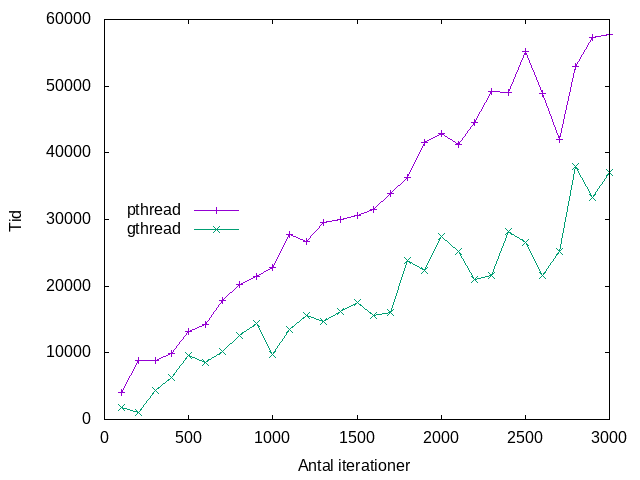
\includegraphics[width=8cm]{benchmarks/mutextest.png}
          \caption{bmark\_mutex(): Exekveringstid(ticks) / Iterationer}
          \label{fig:Graph}
        \end{figure}
        
        
        
\maketitle
\textbf
    {\\\\4. Analys\\\\}
    Resultaten blev inte vad jag förväntade mig, då mitt bibliotek var märkbart snabbare i både timertestet (Figur 2)  och mutextestet (Figur 3). I yieldtestet (Figur 1) var pthreadbiblioteket snabbare med stor marginal.\\\\
    
Efter att ha funderat på det så skulle jag gissa att mitt bibliotek har mindre overhead då det är så pass mycket mindre än pthreadbiblioteket. Ett exempel på det är min cond\_signal funktion, som innehåller fem rader kod. Jag gissar att den motsvarande pthreadfunktionen är lite längre. \\
    Det påståended säger dock emot resultaten på ett sätt, då mitt bibliotek var snabbare i det test med minst antal funktionsanrop, timertestet, medan pthreadbiblioteket var snabbare i yieldtestet. Vad säger det om skillnaderna mellan de olika biblioteken?

    % Varför fick vi det resultatet

    \maketitle
    \textbf
        {\\\\5. Reflektion\\\\}
        Överlag är jag nöjd med mitt arbete men det finns fortfarande några buggar kvar som orsakar sporadiska segmenteringsfel. För att besvara frågan i slutet av uppgiftsinstruktionerna så hade jag inte sovit gott om detta bibliotek användes i styrsystemet för ett flygplan.

\end{document}
